\documentclass[
  a4paper,
  spanish,
  12pt,
  enlargefirstpage,
]{scrartcl}

\linespread{1.2}
%\setlength{\parindent}{13.2pt}
\setlength{\parindent}{0pt}
\setlength{\parskip}{12pt}

\usepackage{babel}

\usepackage{mathtools}

\usepackage{amssymb}

\usepackage{hyperref}
\usepackage{xcolor}
\hypersetup{%
  colorlinks=true,% hyperlinks will be coloured
}

\newcommand*{\QEDA}{\hfill\ensuremath{\blacksquare}}%

\usepackage[activate={true,nocompatibility},final,tracking=true,factor=1100,stretch=10,shrink=10]{microtype}
\SetTracking{encoding={*}, shape=sc}{0}

\usepackage{enumitem}
\setlist[itemize]{leftmargin=*, noitemsep, topsep=0pt}
\setlist[enumerate]{leftmargin=*}

\usepackage{changepage}

\usepackage{lipsum}
\usepackage{amsthm}

\usepackage[labelfont=sc]{caption}
\usepackage{subcaption}
\usepackage{graphicx}

\usepackage{commath}

\usepackage{tikz}
\usetikzlibrary{babel}

\usepackage{float}

\usepackage{listings}
\usepackage{color}
\renewcommand{\lstlistingname}{Listado}

\definecolor{dkgreen}{rgb}{0,0.6,0}
\definecolor{gray}{rgb}{0.5,0.5,0.5}
\definecolor{mauve}{rgb}{0.58,0,0.82}

\lstset{frame=tb,
  language=Python,
  aboveskip=3mm,
  belowskip=3mm,
  showstringspaces=false,
  columns=flexible,
  basicstyle={\small\ttfamily},
  numbers=none,
  numberstyle=\tiny\color{gray},
  keywordstyle=\color{blue},
  commentstyle=\color{dkgreen},
  stringstyle=\color{mauve},
  breaklines=true,
  breakatwhitespace=true,
  tabsize=2
}

\renewcommand{\lstlistingname}{Listado}

%----------------------------------------------------------------------------------------
%	TITLE SECTION
%----------------------------------------------------------------------------------------

\newcommand{\horrule}[1]{\rule{\linewidth}{#1}} % Create horizontal rule command with 1 argument of height

\title{
\normalfont \normalsize
\textsc{Universidad de Granada}\\ [25pt] % Your university, school and/or department name(s)
\horrule{0.5pt}\\ [0.4cm] % Thin top horizontal rule
{\sffamily\bfseries\Large Práctica 2}\\ [6pt] % The assignment title
\textsf{\textsc{Aprendizaje Automático}\\ Doble Grado en Ingeniería Informática y Matemáticas}\
\horrule{2pt}\\ [0.5cm] % Thick bottom horizontal rule
}

\author{Guillermo Galindo Ortuño} % Your name

\date{\normalsize\today} % Today's date or a custom date

\usepackage{blindtext}

\begin{document}

\maketitle % Print the title
\section{Ejercicio sobre la complejidad de H y el ruido}%
\label{sec:ejercicio_sobre_la_complejidad_de_h_y_el_ruido}
En este apartado estudiaremos la complejidad que añade la aparición de ruido en las etiquetas a la hora de elegir la clase de funciones más adecuada.

\subsection{Nube de puntos de ejemplo}%
\label{sub:nube_de_puntos_de_ejemplo}

En primer lugar mostramos dos nubes de puntos generadas con las funciones proporcionadas \texttt{simula\_unif} y \texttt{simula\_gaus}. Como ya dijimos, ambas tomas como parámetros el número de elemtos a generar \texttt{N}, la dimensión de estos \texttt{dim}, y por último el intervalo en el que generarlos o sigma respectivamente.

Dicho esto, para \texttt{simula\_unif} usamos los parámetros \texttt{N=50, dim=2, rango=[-50,50]}, y para \texttt{simula\_gaus} usamos \texttt{N=50, dim=2, sigma=[5,7]}. Los resultados obtenidos los mostramos en las figuras \ref{fig:img/NubeUniforme} y \ref{fig:img/NubeGauss} respectivamente.

\begin{figure}[h]
    \centering
    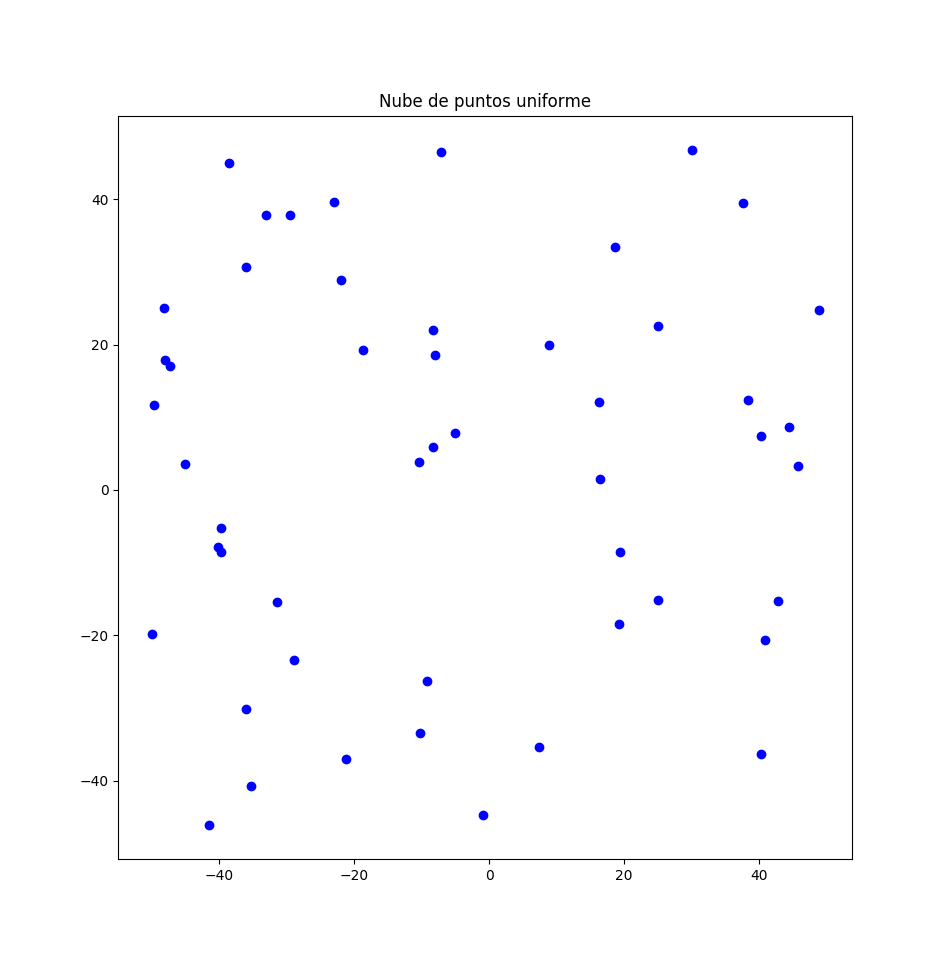
\includegraphics[width=0.6\linewidth]{img/NubeUniforme.png}
    \caption{Nube de puntos generada utilizando una distribución uniforme}%
    \label{fig:img/NubeUniforme}
\end{figure}

\begin{figure}[h]
    \centering
    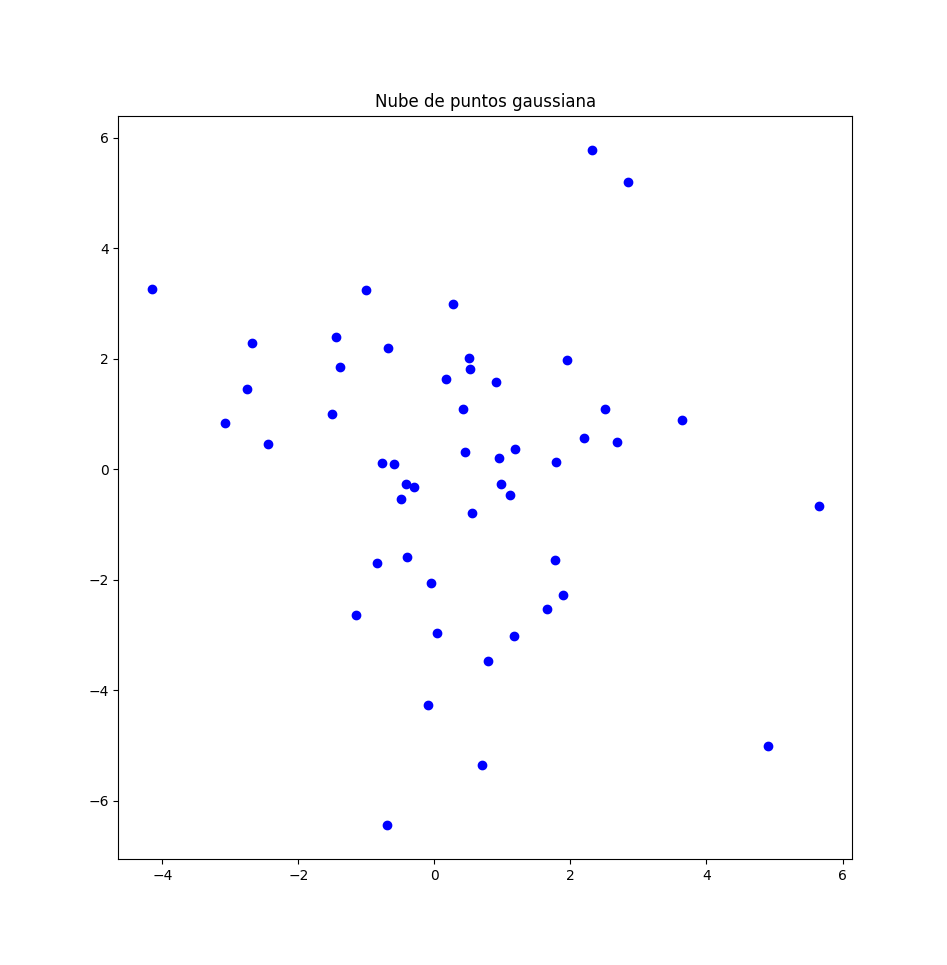
\includegraphics[width=0.6\linewidth]{img/NubeGauss.png}
    \caption{Nube de puntos generada utilizando una distribución gaussiana}%
    \label{fig:img/NubeGauss}
\end{figure}

\subsection{Estudio de la influencia del ruido}%
\label{sub:estudio_de_la_influencia_del_ruido}
En este apartado, en primer lugar generaremos una muestra de puntos 2D a los que añadiremos una etiqueta utilizando el signo de la distancia de dichos puntos a una recta. Para generar los puntos llamaremos a \texttt{simula\_unif(100, 2, [-50,50])}, y para generar la recta para las etiquetas utilizaremos \texttt{simula\_recta([-50, 50])}. A continuación, etiquetaremos cada elemento utilizando el signo de la función \(f(x,y) = y - ax -b\).

Todo esto se encuentra encapsulado en la función \texttt{genera\_datos}, que toma como parametros el número de elementos a generar, la dimensión de estos, y el intervalo en que generarlos. Esta, calcula el conjunto de datos con estos parámetros, genera una recta en dicho intervalo, y etiqueta todos los puntos.

\subsubsection*{Apartado a}%
\label{sub:apartado_a}

A continuación mostramos todos los puntos generados correctamente etiquetados junto con la recta utilizada para ello, en la figura \ref{fig:img/Labes}.

\begin{figure}[h]
    \centering
    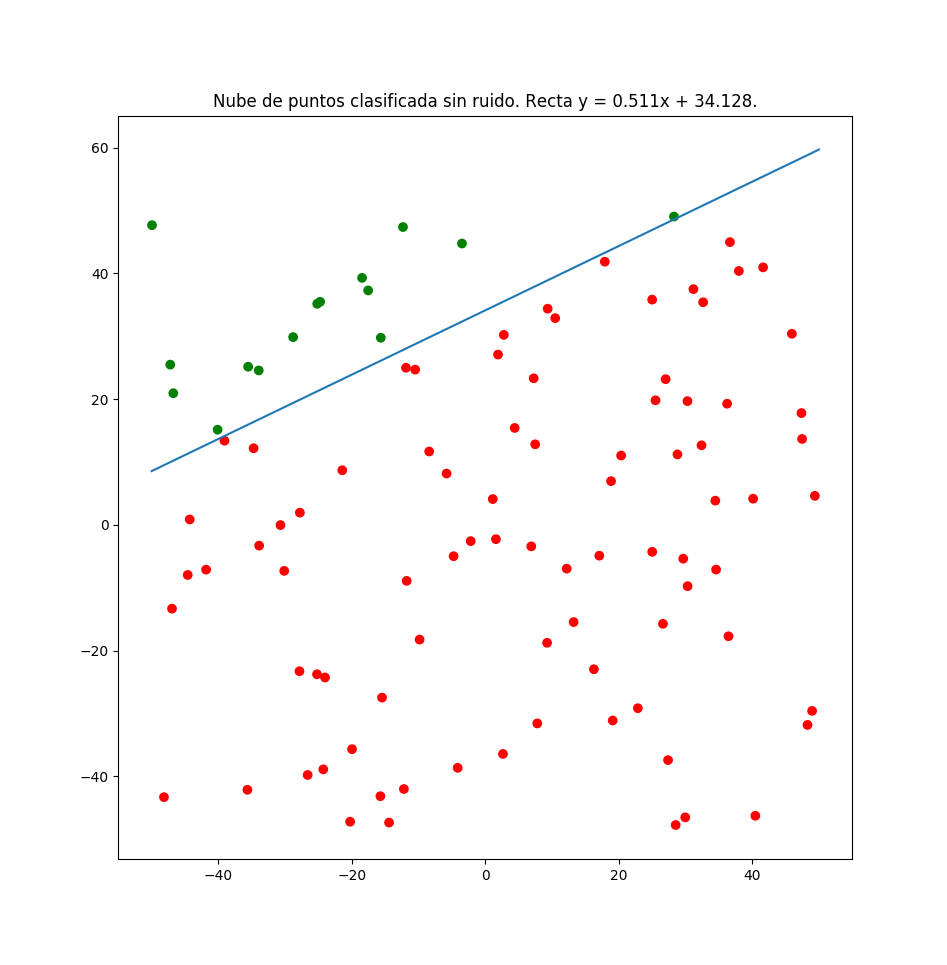
\includegraphics[width=0.6\linewidth]{img/Labes.png}
    \caption{Nube de puntos clasificada con la recta indicada}%
    \label{fig:img/Labes}
\end{figure}

\subsubsection*{Apartado b}%
\label{sub:apartado_b}

Procedemos entonces a añadir ruido en las etiquetas de dichos datos. Para ello modificaremos de forma aleatoria un 10\% de las etiquetas positivas y otro 10\% de las negativas. Los resultados se encuentran en la figura \ref{fig:img/LabelsNoise}, y podemos observar como efectivamente dejan de estar todos los puntos bien clasificados respecto de la recta indicada.

\begin{figure}[h]
    \centering
    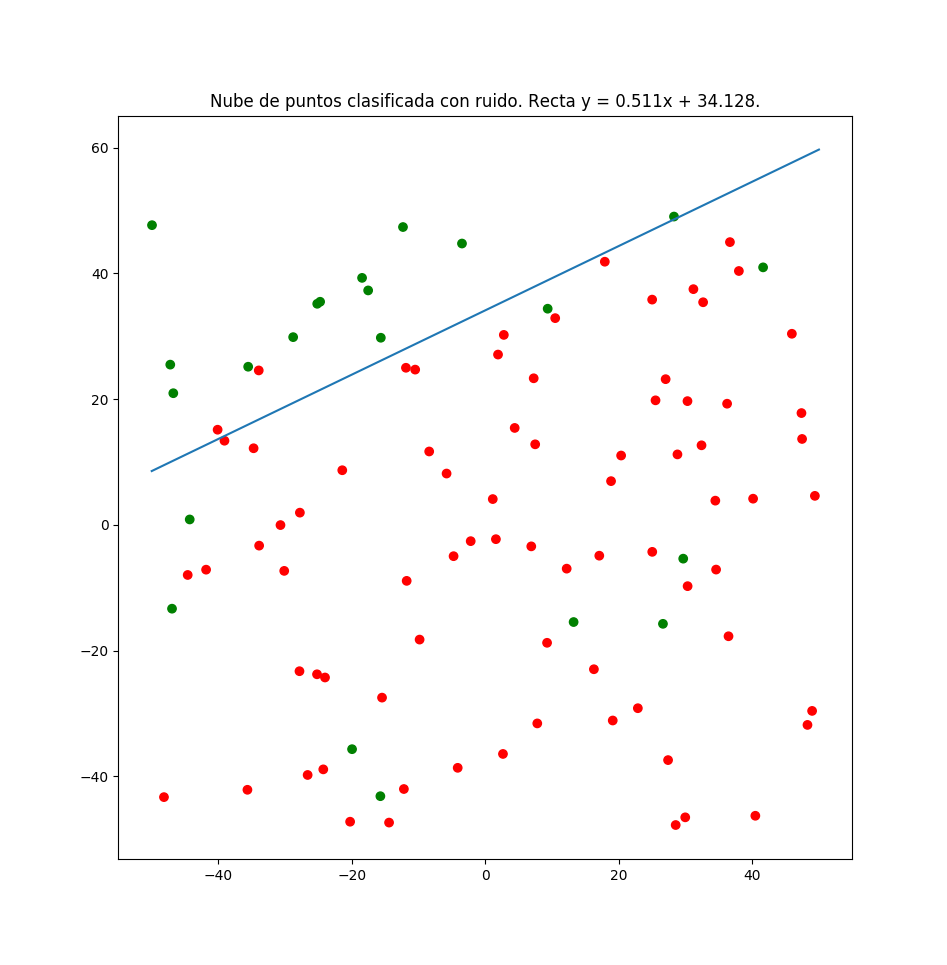
\includegraphics[width=0.6\linewidth]{img/LabelsNoise.png}
    \caption{Nube de puntos clasificada con la recta indicada tras añadir ruido}%
    \label{fig:img/LabelsNoise}
\end{figure}

\subsubsection*{Apartado c}%
\label{sub:apartado_c}
En este apartado utilizaremos cuatro funciones proporcionadas para definir la frontera de clasificación de los puntos de nuestra muestra en lugar de la recta. Estas funciones son:

\begin{itemize}
    \item \(f_1j(x, y) = (x-10)^2 + (y-20)^2 - 400\)
    \item \(f_2(x, y) = 0.5(x+10)^2 + (y-20)^2 - 400\)
    \item \(f_3(x, y) = 0.5(x-10)^2 - (y+20)^2 - 400\)
    \item \(f_4(x,y) = y -20x^2 - 5x + 3\)
\end{itemize}

En primer lugar mostramos las regiones respecto de la recta original (\ref{fig:img/RegRecta}), y las obtenidas usando las funciones recién mencionadas (\ref{fig:sub1}, \ref{fig:sub2}, \ref{fig:sub3}, \ref{fig:sub4}). Para concluir, mostramos los resultados obtenidos al calcular el error de clasificación, es decir, el porcentaje de elementos mal clasificados, que en nuestro caso coincide con el número de elementos mal clasificados pues nuestra muestra es de tamaño 100.

\begin{figure}[h]
    \centering
    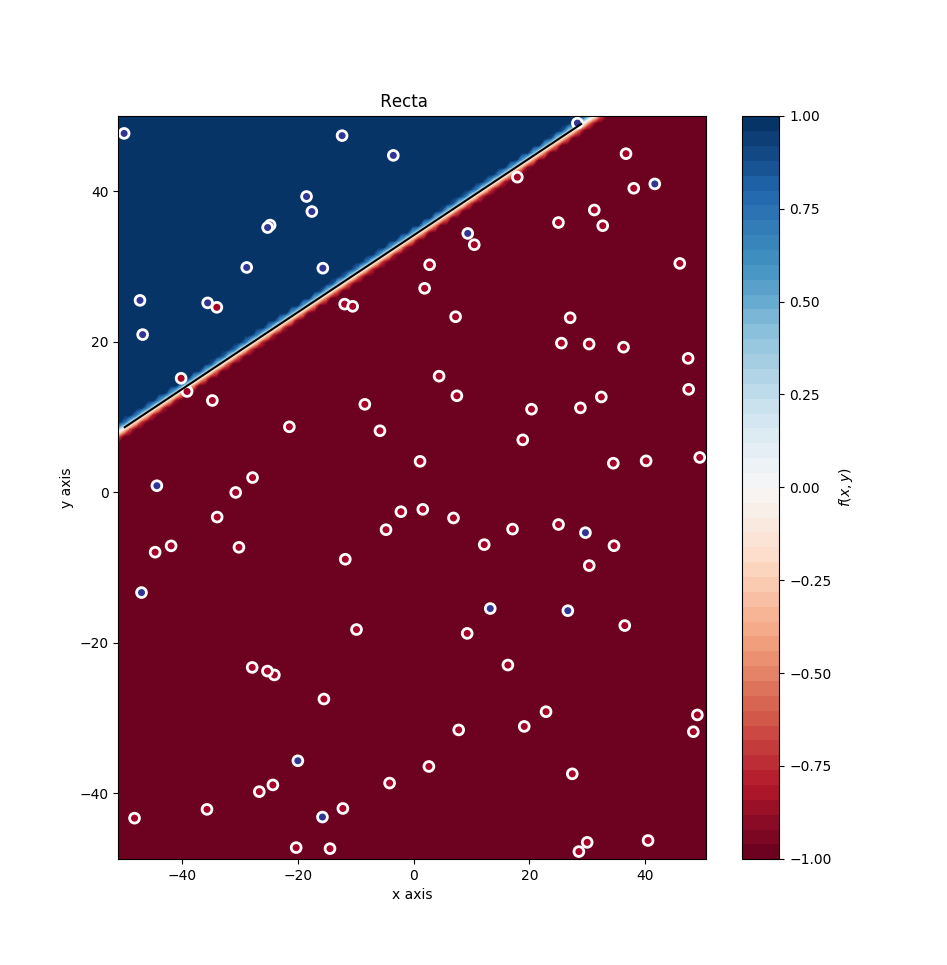
\includegraphics[width=0.6\linewidth]{img/RegRecta.png}
    \caption{Regiones utilizando la recta original}%
    \label{fig:img/RegRecta}
\end{figure}

\begin{figure}
\centering
\begin{subfigure}{0.5\textwidth}
  \centering
  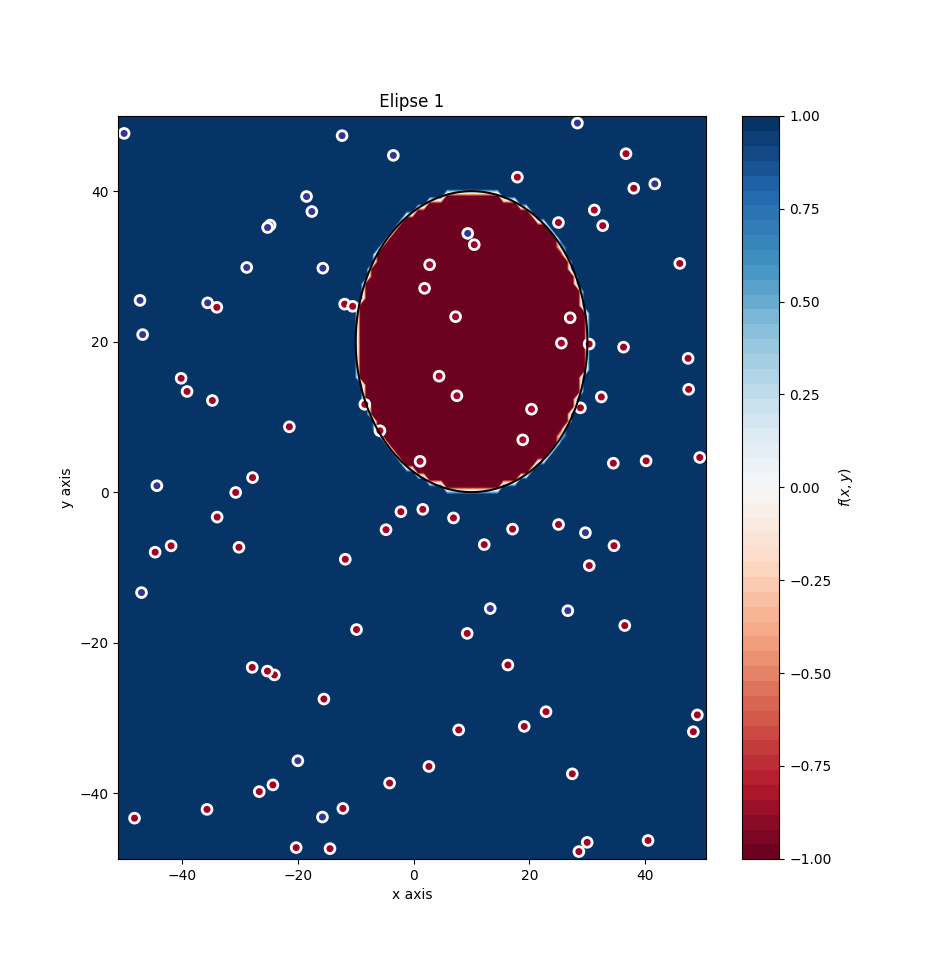
\includegraphics[width=\linewidth]{img/RegElipse1.png}
  \caption{Regiones usando \(f_1\)}
  \label{fig:sub1}
\end{subfigure}%
\begin{subfigure}{.5\textwidth}
  \centering
  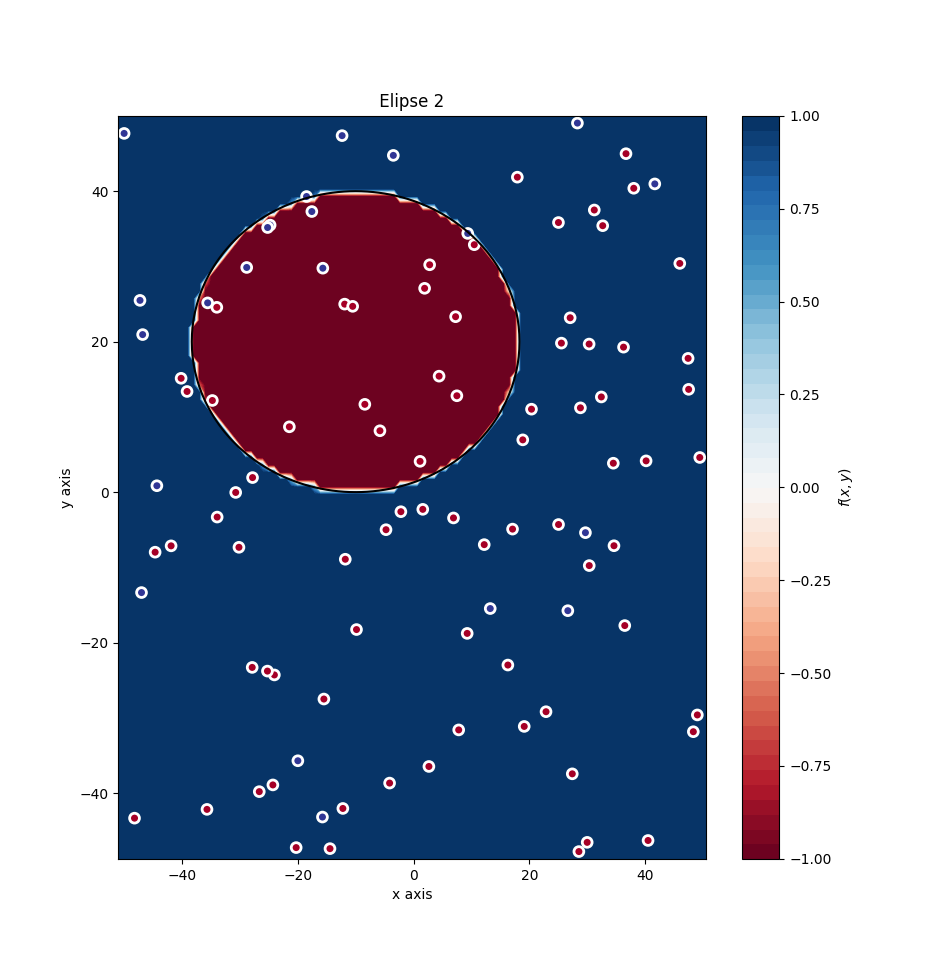
\includegraphics[width=\linewidth]{img/RegElipse2.png}
  \caption{Regiones usando \(f_2\)}
  \label{fig:sub2}
\end{subfigure}
\begin{subfigure}{0.5\textwidth}
  \centering
  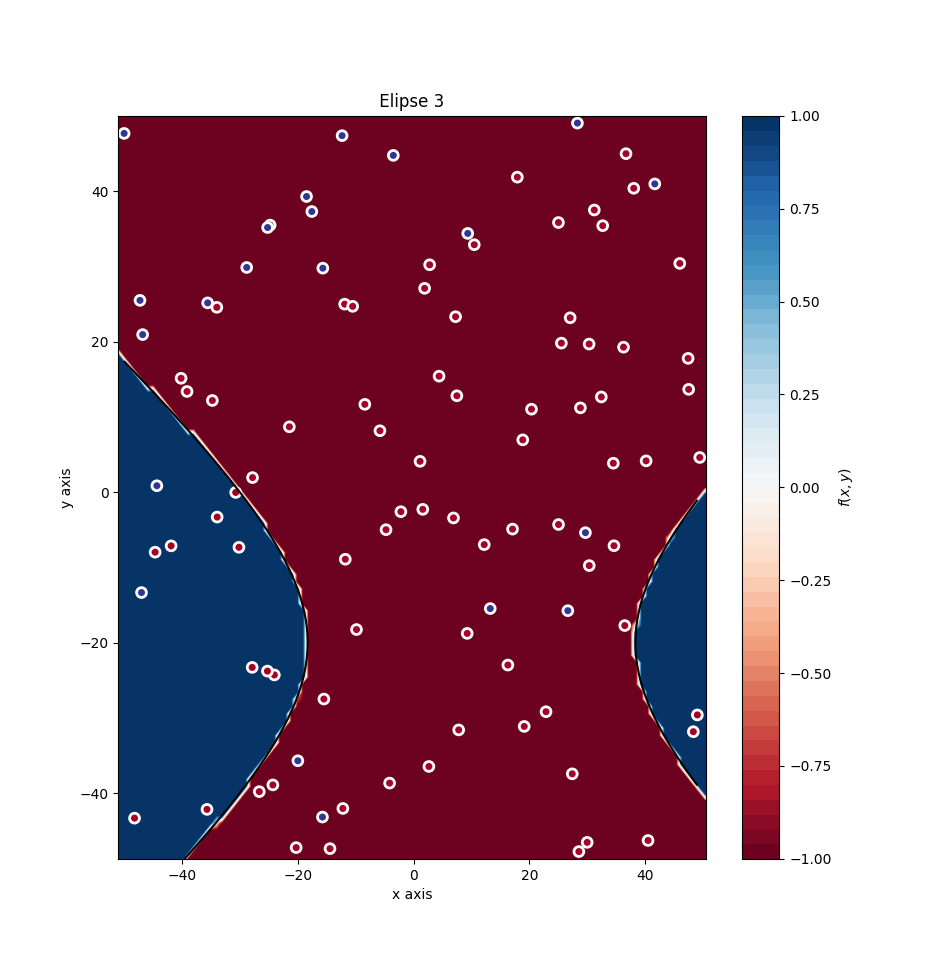
\includegraphics[width=\linewidth]{img/RegElipse3.png}
  \caption{Regiones usando \(f_3\)}
  \label{fig:sub3}
\end{subfigure}%
\begin{subfigure}{.5\textwidth}
  \centering
  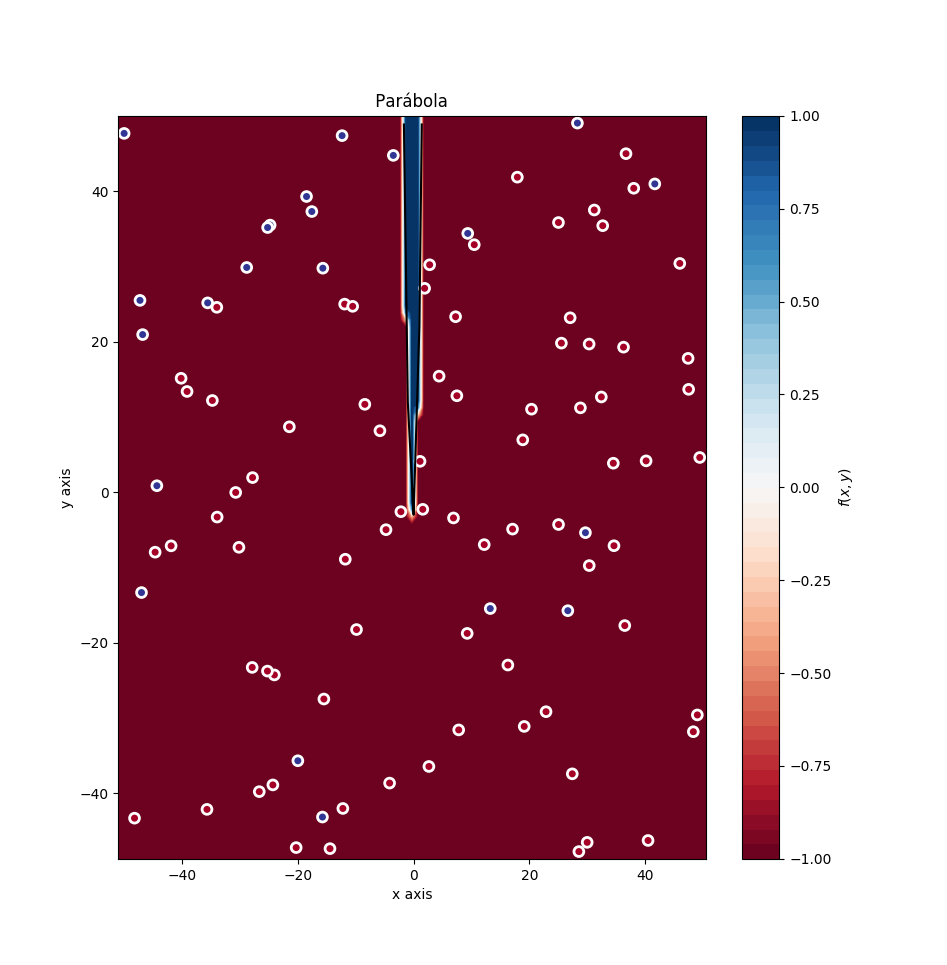
\includegraphics[width=\linewidth]{img/RegParabola.png}
  \caption{Regiones usando \(f_4\)}
  \label{fig:sub4}
\end{subfigure}

\label{fig:reg1}
\end{figure}

% TODO Añadir una conclusión más y mostrar los errores
Como podemos observar tanto en las imágenes como en los errores de clasificación obtenidos, ninguna de estas funciones clasifica nuestra muestra mejor que la recta original.

\section{Modelos lineales}%
\label{sec:modelos_lineales}
Para este apartado utilizaremos dos métodos distintos para encontrar el hiperplano solución a un problema de clasificación binaria. Estos son el algoritmo perceptrón y la regresión logística.

Para en primer lugar hemos implementado el algoritmo de aprendizaje del perceptrón en la función \texttt{ajusta\_PLA}. Esta toma cómo parámetros:
\begin{itemize}
    \item \texttt{datos} : matriz con los datos (en coordenadas homogéneas).
    \item \texttt{labels} : vector de etiquetas.
    \item \texttt{max\_iter}  : máximo de iteraciones permitidas.
    \item \texttt{vini} : valor inicial.
\end{itemize}

Y devuelve:
\begin{itemize}
    \item \texttt{w}: vector de pesos del hiperplano solución.
    \item \texttt{iters}: número de iteraciones realizadas.

\end{itemize}

A continuación mostramos la implementación:

\begin{lstlisting}[]
def ajusta_PLA(datos, labels, max_iter, vini):
    w  = vini.copy()

    for i in range(max_iter):
        w_old = w.copy()

        for item, label in zip(datos, labels):
            if signo(w.dot(item)) != label:
                w += label * item
        if np.all(w == w_old):
            return w, i+1

    return w, i+1

\end{lstlisting}

Lo primero que podemos observar del algoritmo es que determinista, es decir, que siempre que no cambiemos los parámetros, el resultado será el mismo pues no hay ninguna componenente aleatoria.

\subsection{Resultados utilizando datos sin ruido}%
\label{sub:resultados_utilizando_datos_sin_ruido}
Aquí utilizaremos los datos generados en \ref{sub:apartado_a}. Estos son los datos sin la modificación de las etiquetas que simulan el ruido. Lo ejecutamos una vez con vector inicial \([0,0,0]\), y otras diez veces con vectores con valores aleatorios en el intervalo \([0,1]\). Con el vector \(0\) solo le ejecutamos una vez pues, como ya dijimos, el algoritmo es determinista y por tanto si no cambiamos nada el resultado seguiría siendo el mismo.\\

Los resultados que hemos obtenido son los siguientes:

\end{document}
